\section{Exercise : Application of MCFP - Rectilinear planar embedding}

\subsection{Values of $z_{fg}$ and $x_{vf}$, total breakpoints, and rectilinear graph}

The values of $z_{fg}$ are given in figure \ref{fig:zfgtable}. The values of $x_{vf}$ are given in figure \ref{fig:xvftable}.

\begin{figure}
\centering
\begin{tabular}{l|lllll}
$z_{fg}$ & $a$ & $b$ & $c$ & $d$ & $e$  \\ \hline
$a$ & - & $z_{ab} = 0$ & $z_{ac} = 0$ & $z_{ad} = 0$ & $z_{ae} = 0$ \\
$b$ & $z_{ba} = 2$ & - & $z_{bc} = 1$ & $z_{bd} = 1$ & $z_{be} = 0$ \\
$c$ & $z_{ca} = 1$ & $z_{cb} = 1$ & - & $z_{cd} = 0$ & $z_{ce} = 0$ \\
$d$ & $z_{ad} = 0$ & $z_{db} = 1$ & $z_{dc} = 0$ & - & $z_{de} = 2$ \\
$e$ & $z_{ea} = 4$ & $z_{eb} = 0$ & $z_{ec} = 0$ & $z_{ed} = 0$ & - \\
\end{tabular}
\caption{\label{fig:zfgtable}Values of $z_{fg}$ for all boundary cycles $f$ and $g$ in figure 3 of the assignment text.}
\end{figure}

\begin{figure}
\centering
\begin{tabular}{l|lllllll}
$x_{vf}$ & $a$ & $b$ & $c$ & $d$ & $e$ \\ \hline
$v_1$ & $x_{v_1a} = 0 $ & $x_{v_1b} = 1 $ & $x_{v_1c} = 1 $ & $x_{v_1d} = 0 $ & $x_{v_1e} = 0 $ \\
$v_2$ & $x_{v_2a} = 0 $ & $x_{v_2b} = 0 $ & $x_{v_2c} = 1 $ & $x_{v_2d} = 1 $ & $x_{v_2e} = 0 $ \\
$v_3$ & $x_{v_3a} = 1 $ & $x_{v_3b} = 0 $ & $x_{v_3c} = 1 $ & $x_{v_3d} = 1 $ & $x_{v_3e} = 1 $ \\
$v_4$ & $x_{v_4a} = 0 $ & $x_{v_4b} = 0 $ & $x_{v_4c} = 0 $ & $x_{v_4d} = -1 $ & $x_{v_4e} = 1 $ \\
$v_5$ & $x_{v_5a} = 1 $ & $x_{v_5b} = 0 $ & $x_{v_5c} = 0 $ & $x_{v_5d} = 0 $ & $x_{v_5e} = -1 $ \\
$v_6$ & $x_{v_6a} = 1 $ & $x_{v_6b} = 1 $ & $x_{v_6c} = 0 $ & $x_{v_6d} = 1 $ & $x_{v_6e} = 1 $ \\
$v_7$ & $x_{v_7a} = 0 $ & $x_{v_7b} = 0 $ & $x_{v_7c} = 0 $ & $x_{v_7d} = 0 $ & $x_{v_7e} = 0 $ \\
\end{tabular}
\caption{\label{fig:xvftable}Values of $x_{vf}$ for all boundary cycles $f$ and vertices $v$ in figure 3 of the assignment text.}
\end{figure}

The total number of breakpoints in the graph of figure 3 is:

$$ \sum_{f\in F} \sum_{g \in F \setminus{\{f\} }} {z_{fg} + z_{gf} }= 13$$

A rectilinear layout of the graph from figure $2$ in the assignment text is given in figure \ref{fig:reclayout}.

\begin{figure}
 \centering
 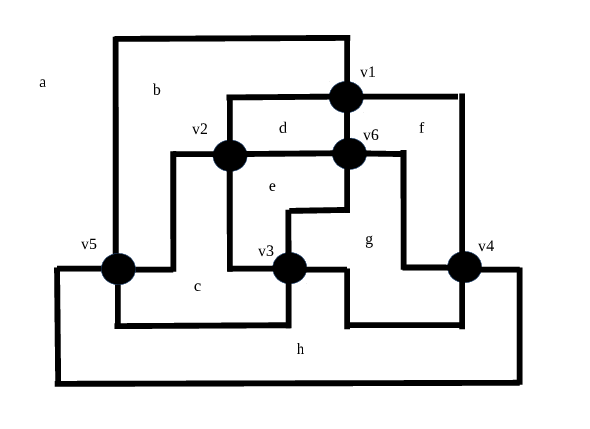
\includegraphics[keepaspectratio=true, width=80mm]{img/rectilinear_graph.png}
 % rectilinear graph.png: 590x429 pixel, 95dpi, 15.77x11.47 cm, bb=0 0 447 325
 \caption{Rectilinear graph of figure 2 in assignment.}
 \label{fig:reclayout}
\end{figure}

\pagebreak

\subsection{Statement of linear constraints and verification}
$F$: is defined as the set of boundary cycles

One constraint per face $f \in F$
$$\sum_{v \in V}{x_{vf}} + \sum_{g \neq f \in F}{z_{fg}} - \sum_{g \neq f \in F}{z_{gf}} =
\begin{cases} -4 & \text{if $f$ is external} \\ 4 & \text{if $f$ is internal}\end{cases}
$$

\textbf{Verify constraints for faces $a$ and $e$}

\textbf{face $a$}
\begin{align*}
  f_{\text{external}}: -4
  &= (x_{v_1a}+x_{v_3a}+x_{v_5a}+x_{v_6a}+x_{v_7a})
   + (z_{ab} + z_{ac} + z_{ae}) - (z_{ba} + z_{ca} + z_{ea})\\
  &= (0+1+1+0+1) + (0+0+0) - (2+1+4)  = 3 + 0 - 7 = -4
\end{align*}

\textbf{face $e$}
\begin{align*}
  f_{\text{internal}}: 4
  &= (x_{v_3,e}+x_{v_4,e}+x_{v_5,e}+x_{v_6,e}+x_{v_7,e})
   + 2 \cdot (z_{e,a} + z_{e,d})\\
  &- (|E_{v_3,v_4}| + |E_{v_3,v_5}| + |E_{v_4,v_6}| + |E_{v_5,v_7}| + |E_{v_6,v_7}|) \\
  &= (1+1-1+1+0) + 2 \cdot (4+0) - (1+2+1+1+1)  = 2 + 2 \cdot 4 - 6 = 4
\end{align*}



\subsection{Nessecary assumption, show that $\sum x_{vf}$ holds}

The assumption that no vertex has degree larger than 4 comes from the 'planar' embedding, thus in 2 dimensions only 2 orthogonal directions are available, lets call them north/south, which we define to be parallel with the y-axis, and east/west defined parallel to the x-axis. When these directions are relative to a vertex, this number doubles, from the point of view of the vertex there are now 4 directions to go, or \textit{degrees}: north, south east and west. If we were to use a 'spatial' embedding, an extra dimension would be added, allowing for 6 degrees (adding up and down).

to be done:show that $\sum{x_{vf}}$ holds for all vertices

To show that this equation holds, we demonstrate it case wise, and rest upon the fact that mirroring in any or both of the principal axis, along with rotating around the vertex in either direction (clockwise or counterclockwise) with any multiplum of $\frac{\pi}{2}$ yields the same result, covering all the possible cases in rectilinear planar embedding.
\begin{figure}[h]
\centering
  \begin{tikzpicture}[line cap=round,line join=round,>=triangle 45,x=1.0cm,y=1.0cm]
    \clip(2,0) rectangle (14.5,4.5);
    \draw[color=qqwuqq,fill=qqwuqq,fill opacity=0.1] (3.39,2) -- (3.39,2.39) -- (3,2.39) -- (3,2) -- cycle; 
    \draw [shift={(3,2)},color=qqwuqq,fill=qqwuqq,fill opacity=0.1] (0,0) -- (-270:0.45) arc (-270:0:0.45) -- cycle;
    \draw[color=qqwuqq,fill=qqwuqq,fill opacity=0.1] (7.89,2) -- (7.89,2.39) -- (7.5,2.39) -- (7.5,2) -- cycle; 
    \draw[color=qqwuqq,fill=qqwuqq,fill opacity=0.1] (7.5,2.39) -- (7.11,2.39) -- (7.11,2) -- (7.5,2) -- cycle; 
    \draw [shift={(7.5,2)},color=qqwuqq,fill=qqwuqq,fill opacity=0.1] (0,0) -- (-180:0.45) arc (-180:0:0.45) -- cycle;
    \draw[color=qqwuqq,fill=qqwuqq,fill opacity=0.1] (12.39,2) -- (12.39,2.39) -- (12,2.39) -- (12,2) -- cycle; 
    \draw[color=qqwuqq,fill=qqwuqq,fill opacity=0.1] (12,2.39) -- (11.61,2.39) -- (11.61,2) -- (12,2) -- cycle; 
    \draw[color=qqwuqq,fill=qqwuqq,fill opacity=0.1] (11.61,2) -- (11.61,1.61) -- (12,1.61) -- (12,2) -- cycle; 
    \draw[color=qqwuqq,fill=qqwuqq,fill opacity=0.1] (12,1.61) -- (12.39,1.61) -- (12.39,2) -- (12,2) -- cycle; 
    \draw [line width=1.6pt] (3,2)-- (3,4);
    \draw [line width=1.6pt] (3,2)-- (5,2);
    \draw (3.29,3.36) node[anchor=north west] {$x_{vf_1} = 1$};
    \draw (3,1.08) node[anchor=north west] {$x_{vf_2} = -1$};
    \draw [line width=1.6pt] (7.5,2)-- (7.5,4);
    \draw [line width=1.6pt] (7.5,2)-- (9.5,2);
    \draw (7.79,3.38) node[anchor=north west] {$x_{wf_1} = 1$};
    \draw (6.96,0.93) node[anchor=north west] {$x_{wf_2} = 0$};
    \draw [line width=1.6pt] (7.5,2)-- (5.5,2);
    \draw (5.51,3.36) node[anchor=north west] {$x_{wf_3} = 1$};
    \draw [line width=1.6pt] (12,2)-- (12,4);
    \draw [line width=1.6pt] (12,2)-- (14,2);
    \draw [line width=1.6pt] (12,2)-- (10,2);
    \draw (10.32,3.34) node[anchor=north west] {$x_{qf_1} = 1$};
    \draw [line width=1.6pt] (12,2)-- (12,0);
    \draw (12.41,3.28) node[anchor=north west] {$x_{qf_2} = 1$};
    \draw (10.26,0.92) node[anchor=north west] {$x_{qf_3} = 1$};
    \draw (12.72,0.86) node[anchor=north west] {$x_{qf_4} = 1$};
    \begin{scriptsize}
    \fill [color=qqqqff] (3,2) circle (1.5pt);
    \draw[color=qqqqff] (2.75,2.09) node {$v$};
    \fill [color=qqqqff] (3,4) circle (1.5pt);
    \draw[color=qqqqff] (3.14,4.13) node {$v_1$};
    \fill [color=qqqqff] (5,2) circle (1.5pt);
    \draw[color=qqqqff] (5.14,2.14) node {$v_2$};
    \draw[color=qqwuqq] (3.77,2.22) node {$90\textrm{\degre}$};
    \draw[color=qqwuqq] (3.74,1.81) node {$270\textrm{\degre}$};
    \fill [color=qqqqff] (7.5,2) circle (1.5pt);
    \draw[color=qqqqff] (7.41,1.87) node {$w$};
    \fill [color=qqqqff] (7.5,4) circle (1.5pt);
    \draw[color=qqqqff] (7.65,4.13) node {$w_1$};
    \fill [color=qqqqff] (9.5,2) circle (1.5pt);
    \draw[color=qqqqff] (9.65,2.14) node {$w_2$};
    \draw[color=qqwuqq] (8.28,2.31) node {$90\textrm{\degre}$};
    \fill [color=qqqqff] (5.5,2) circle (1.5pt);
    \draw[color=qqqqff] (5.67,2.22) node {$w_3$};
    \draw[color=qqwuqq] (6.56,2.34) node {$90\textrm{\degre}$};
    \draw[color=qqwuqq] (8.29,1.72) node {$180\textrm{\degre}$};
    \fill [color=qqqqff] (12,2) circle (1.5pt);
    \draw[color=qqqqff] (11.75,2.25) node {$q$};
    \fill [color=qqqqff] (12,4) circle (1.5pt);
    \draw[color=qqqqff] (12.15,4.13) node {$q_1$};
    \fill [color=qqqqff] (14,2) circle (1.5pt);
    \draw[color=qqqqff] (14.15,2.14) node {$q_2$};
    \draw[color=qqwuqq] (12.79,2.39) node {$90\textrm{\degre}$};
    \fill [color=qqqqff] (10,2) circle (1.5pt);
    \draw[color=qqqqff] (10.18,2.22) node {$q_3$};
    \draw[color=qqwuqq] (11.04,2.32) node {$90\textrm{\degre}$};
    \fill [color=qqqqff] (12,0) circle (1.5pt);
    \draw[color=qqqqff] (12.15,0.14) node {$q_4$};
    \draw[color=qqwuqq] (11.05,1.7) node {$90\textrm{\degre}$};
    \draw[color=qqwuqq] (12.82,1.71) node {$90\textrm{\degre}$};
    \end{scriptsize}
  \end{tikzpicture}
  \caption{3 general situations of total amount of x}
  \label{fig:sumofx}
\end{figure}

\textbf{Case $v$ has degree 2:} one inner and one outer turn is present, yielding $\sum_f{x_{vf}} = 1 - 1 = 0$

\textbf{Case $v$ has degree 3:} two inner turn and one 'otherwise' is present, yielding $\sum_f{x_{vf}} = 1 + 1 + 0 = 2$

\textbf{Case $v$ has degree 4:} four inner turns are present, yielding $\sum_f{x_{vf}} = 1 + 1 + 1 + 1 = 4$

\subsection{Formulate objective function, and linear program with constraints}

The objective function would be Minimizing
$$ \sum_{f\in F} \sum_{g \in F \setminus{\{f\} }} {z_{fg} + z_{gf} }$$

subject to the following constraints

For each face $f \in F$ (from ex 2.2)
$$\sum_{v \in V}{x_{vf}} + \sum_{g \neq f \in F}{z_{fg}} - \sum_{g \neq f \in F}{z_{gf}} = \begin{cases} -4 & \text{if $f$ is external} \\ 4 & \text{if $f$ is internal}\end{cases}
$$

For each vertex $v \in V$ (from ex 2.3)
$$  \sum_{f \in F} {x_{vf}} = \begin{cases}
                                0 & \text{if $v$ has degree } 2 \\
                                2 & \text{if $v$ has degree } 3 \\
                                4 & \text{if $v$ has degree } 4
                              \end{cases}
$$

All $z_{fg}$ are non negative
$$ z_{fg} \ge 0 \quad \forall f, g \in F, \:f\neq g $$

\subsection{Rewrite to an instance of MCFP}

Intuitively, we want the vertices in the MCFP instance to correspond to the faces of the rectilinear layout. The external face has a demand of $-4$, and all internal faces have a demand of $4$. Inner turns are represented as flow into the vertex, and outer turns as flow out of the vertex.

Turns on breakpoints are represented as edges from one face to another. To represent turns on vertices from the rectilinear layout, we add more vertices to the MCFP intstance; one for each vertex in the rectilinear layout. The demand of such a vertex is always negative, and corresponds to the number of faces that have inner turns on that vertex. For vertex $v$, that's exactly $-\sum_{f \in F}{x_{vf}}$.

\textbf{In this graph:} \\
Nodes represent face cycles $f \in F$, and nodes $v_i \in V$.\\
Edges between face and vertex nodes represent 'locked' breakpoints, $x_{fv}$, they are black. Are they locked??\\
Edges between faces represent 'free' breakpoints $z_{fg}$, they are blue in the graph. These are to be minimized.

Any negative edges, is reversed and multiplied by $-1$ (such as $x_{v_4d}=-1 \rightarrow x_{dv_4}=1)$.\\
Antiparallel edges $b \leftrightarrow c$ are fixed by inserting an extra node $b'$.
\begin{figure}[h]
    \centering
    \begin {tikzpicture}[-latex, auto, node distance=36mm and 48mm ,on grid ,
                          semithick ,
                          main node/.style ={ circle , color=white ,
                          draw , black , text=black , minimum width =8mm}]

      \node[main node] (a) [label=above right:$a$]{$-4$};
      \node[main node] (b) [above =of a, label=above left:$b$] {$4$};
      \node[main node] (bc) [node distance=15mm and 28 mm,below right =of b, label=above right:$b'$] {$0$};
      \node[main node] (c) [right =of a, label=above right:$c$] {$4$};
      \node[main node] (d) [below =of a, label=above right:$d$] {$4$};
      \node[main node] (e) [left =of a, label=below left:$e$] {$4$};
      \node[main node] (v1) [above =of c, label=above left:$v_1$] {$-2$};
      \node[main node] (v2) [below =of c, label=above left:$v_2$] {$-2$};
      \node[main node] (v3) [left =of d, label=above left:$v_3$] {$-2$};
      \node[main node] (v4) [left =of e, label=above left:$v_4$] {$0$};
      \node[main node] (v5) [above left =of e, label=above left:$v_5$] {$0$};
      \node[main node] (v6) [above =of e, label=above left:$v_6$] {$-4$};
      \node[main node] (v7) [below left =of e, label=above left:$v_7$] {$0$};

    \color{blue}
    \path[every node/.style={font=\sffamily\small}]
    (b)  edge node {$z_{ba}=2$} (a)
%          edge [bend left=10] node {$1$} (c)
         edge node {$1$} (bc) %
         edge [bend left, below right] node {$1$} (d)

    (bc) edge node {$1$} (c) %
         
    (c)  edge [above] node {$1$} (a)
         edge [bend left=10] node {$1$} (b)
        
    (d)  edge [bend left, below left] node {$1$} (b)
         edge [bend left=10, above] node {$2$} (e)

    (e)  edge node {$4$} (a)
    ;
    \color{black}
    \path[every node/.style={font=\sffamily\small}]
    (d)  edge [above left] node {$1$} (v4) % reversed
    (e)  edge [below left] node {$1$} (v5) % reversed

    (v1) edge node {$x_{v_1b}=1$} (b)
         edge node {$1$} (c)

    (v2) edge node {$1$} (c)
         edge node {$1$} (d)

    (v3) edge [bend left=10, above] node {$1$} (a)
         edge node {$1$} (c)
         edge node {$1$} (d)
         edge [below right] node {$1$} (e)

    (v4) %edge node {$-1$} (d)
         edge node {$1$} (e)

    (v5) edge [below left] node {$1$} (a)
         %edge [below left] node {$-1$} (e)
         
    (v6) edge node {$1$} (a)
         edge node {$1$} (b)
         edge [bend right=10, left] node {$1$} (d)
         edge node {$1$} (e)
         ;
    \end{tikzpicture}
    \caption{MCFP graph of the rectilinear planar problem}
    \label{fig:ex2a}
\end{figure}

